\documentclass[a4paper,10pt]{scrreprt}
\usepackage[top=2cm,bottom=2cm,left=2cm,right=2cm]{geometry}
\usepackage[utf8]{inputenc}
\usepackage{graphicx}
\usepackage[german]{babel}
\usepackage{pdfpages}
%opening
\title{Enterprise Application Frameworks Teil 2 - MSP}
\author{Roland Hediger}
\usepackage{fancyhdr}
\renewcommand{\familydefault}{\sfdefault}
\newcommand{\pic}[2][figure]{\begin{figure}[h]
 \centering
 \includegraphics[scale=0.3]{#2}
 % rsc.png: 0x0 pixel, 0dpi, 0.00x0.00 cm, bb=
 \caption{#1}
\end{figure}
}
\usepackage{framed}
% Code listenings
\usepackage{color}
\usepackage{xcolor}
\usepackage{listings}
\usepackage{caption}
\usepackage[T1]{fontenc}
\DeclareCaptionFont{white}{\color{white}}
\DeclareCaptionFormat{listing}{\colorbox{gray}{\parbox{\textwidth}{#1#2#3}}}
\captionsetup[lstlisting]{format=listing,labelfont=white,textfont=white}
\lstset{
 language=Java,
 basicstyle=\footnotesize\ttfamily, % Standardschrift
 numbers=left,               % Ort der Zeilennummern
 numberstyle=\tiny,          % Stil der Zeilennummern
 stepnumber=5,              % Abstand zwischen den Zeilennummern
 numbersep=5pt,              % Abstand der Nummern zum Text
 tabsize=2,                  % Groesse von Tabs
 extendedchars=true,         %
 breaklines=true,            % Zeilen werden Umgebrochen
 frame=b,         
 %commentstyle=\itshape\color{LightLime}, Was isch das? O_o
 %keywordstyle=\bfseries\color{DarkPurple}, und das O_o
 basicstyle=\footnotesize\ttfamily,
 stringstyle=\color[RGB]{42,0,255}\ttfamily, % Farbe der String
 keywordstyle=\color[RGB]{127,0,85}\ttfamily, % Farbe der Keywords
 commentstyle=\color[RGB]{63,127,95}\ttfamily, % Farbe des Kommentars
 showspaces=false,           % Leerzeichen anzeigen ?
 showtabs=false,             % Tabs anzeigen ?
 xleftmargin=17pt,
 framexleftmargin=17pt,
 framexrightmargin=5pt,
 framexbottommargin=4pt,
 showstringspaces=false      % Leerzeichen in Strings anzeigen ?        
}

\begin{document}

\maketitle
\tableofcontents
\newpage
 \pagestyle{fancy}
\part{Theorie}

\chapter{Einführung  Enterpise Beans}

\begin{description}
 \item [Definition] Ein Enterprise Bean ist eine serverseitige Komponente die die Businesslogik einer Applikation Kapselt ( Facade).
 \begin{itemize}
  \item Beitet eine externe interface an (Remote)
  \item Versteckt komplexität der Implementation.
 \end{itemize}
\item [Zusätzliche Services] Transaktionsmanagement, Sicherheitsdienste, Concurrency Management.
\end{description}

\section{EJB Component Architecture}
\pic{ejbca.png}

\subsection{Synchrone Enterprise Beans}
\begin{description}
 \item [Stateless Session Bean] Bietet Dienste an, kann ein Webservice Implementieren.Ahnlich wie Spring Beans mit \texttt{scope=Singleton}
 \item [Stateful Session Bean] Instanzvariablen representieren eine einzigartige Client-Bean Session. Ähnlich wie Spring Beans mit \texttt{scope=Prototype}.
\end{description}

\subsection{Asynchrone Enterprise Beans}
\begin{description}
 \item [Message Driven Beans] Haltet die Daten oder der Zustand eines spezifischen Clients nicht. Kann auf JMS basiert sein.
\end{description}

\section{Implementation von Enterprise Beans}
\begin{description}
 \item [Enterprise Bean] Primäre Artifakt. Annotiertes POJO. Die Annotation geben die Semantik sowohl als die Vorraussetzungen an dem EJB Container.
 \item [Enterprise Business Interface] Gewöhnliche Interface. Ein EJB\footnote{Enterprise Java Bean} kann mehrere ``Business Interfaces'' implementieren.\\
 \begin{description}
  \item [Remote Interfaces] \texttt{@Remote} : Entfernte Client kann auf einer anderen JVM laufen. Ort der EJB ist für Client Transparent.
  \item [Local Interfaces] Die müssen \textit{auf der gleichen JVM wie EJB laufen.} Ort ist für den Client nicht Transparent.
  \item [Unterschiede] Performanz, Isolation von Paramter. 
 \end{description}
\item [JNDI Access] \hfill \\
\begin{lstlisting}[caption=JNDI]
 Properties props = new Properties();
props.put(Context.INITIAL_CONTEXT_FACTORY,
"org.jboss.naming.remote.client.InitialContextFactory");
props.put(Context.PROVIDER_URL, "remote://localhost:4447");
props.put(Context.SECURITY_PRINCIPAL, "testuser");
props.put(Context.SECURITY_CREDENTIALS, "testpassword");
context = new InitialContext(props);
context.lookup(...)
\end{lstlisting}

\end{description}

\section{Stateless Session Beans}
\begin{description}
 \item [Eigenschaften.] Bietet ein Dienst an für Clients. Verwaltet keine ``Conversational State'' mit Clients. Ein Stateless Bean kann \textbf{Instanzvariablen beinhalten, aber die sind nur für den Dauer des Aufrufs gültig.} EJB Container kann eine \textbf{beliebige Instanz} der Bean an dem Client geben bei einem Methodenaufruf. Client-to-Bean Assoziation ist daher kurz. Es kann jedoch \textbf{globale Zustandsinformation} beinhalten wie ein JNDI Context oder JDBC Verbindung. Diese Instanz ist nicht geteilt - 1 Client pro Instanz.
\end{description}
\begin{lstlisting}[caption=Calculator Example Stateless Bean]
public interface Calculator {
  double sum (double x, double y);
  double difference (double x, double y);
  double product (double x, double y);
  double quotient (double x, double y);
}
// No interface inheritance - no remote xceptions!

// Implementation

@Stateless
@Remote(value = {Calculator,class})
public class CalculatorBean implements Calculator {
  ...//selbsterklaerend normale implementation.
}

// Client
public class Client {
	public static void main(String[] args throws Exception{
		InitialContext ctx = new InitialContext();
		Calculator calculator = (Calculator) ctx.lookup(
		"calculator/CalculatorBean!calculator.bean.Calculator");
		System.out.println("1 + 1 = "+calculator.add(1, 1));
		System.out.println("1 - 1 = "+calculator.subtract(1, 1));
	}
}
\end{lstlisting}
\begin{description}
 \item [Remarks] Die Stateless Annotation sagt dem EJB Container dass der CalculatorBean Stateless ist. Es hat folgende Eingabeeigenschaften : 
 \begin{itemize}
  \item Name : Names des Beans default : Unqualified Class Name
  \item Description : Muss in tools angezeigt werden - Beschreibung der Bean.
  \item mappedName : mapping to a JNDI Name. 
 \end{itemize}
 \item[@Remote] Ist dann business Interface. Value ist dann spezifiziert falls die Annotation auf eine Klasse angewendet ist. Interface nicht unbedingt durch einer Bean Klasse implementiert. Variante : Interface selbst annotieren.
 \item[@Local] Ist dan ein Local Interface. Funktioniet nicht falls ein Lokale Client auf eine andere VM ist. Mögliche Anwendung - Web Container. \textbf{Das gleiche Business Interface kann nicht gleichzeitig Lokal und Remote sein.}
\end{description}

\begin{framed}
 Bean Implementation muss ein Defaultkonstruktor haben. 
\end{framed}

\section{Statelss Bean Lifecycle}
\pic{slsbl.png}

\section{Callback Methods for Stateless Session Beans}
\begin{description}
 \item[@PostConstruct] Nur einmal auf jeden Instanz nachdem Dependency Injections fertig sind. Aufgerufen bevor Ausführung der ersten Methode. Nur eine methode kann mit dieser Annotation markiert sein.
 \item[@PreDestroy] Aufgerufen wenn der Beaninstanz zerstört ist. Sollte alle Resourcen schliessen, ähnlich wie finalize. Nur eine methode kann mit dieser Annotation markiert sein.
 \item[Bemerkung] Diese Methoden sind in eine \textit{noch nicht spezifizierte} Transaktions und Sicherheitskontext aufgerufen. Annotierte methoden sollen folgende Kritieren erfüllen: 
 \begin{itemize}
  \item Keine Parameter, return type void. Sichtbarkeit ist irrelevant.
  \item Muss keine CheckedExceptions werfen.
 \end{itemize}

\end{description}

\section{Pooling}
Ein Stateless Bean behandelt die Aufrufe von Clients. Kein Conversational State - Keine Abhängigkeit von 
Client.Teilen von ein Bean zwischen Clients bedeutet weniger Resourcen. \textbf{Beans sind Single Threaded}\\
\textbf{Clustering:} Bean Instanzen können auf mehrere Server sein.

Entfernung der Instanz von einem Stateless Bean ist transparent und von Container behandelt.


\section{EJB Reuse - Dependency Injection}
\begin{framed}
\begin{verbatim}
  beanRemoteInterface = (Foo) ctx.lookup("myapp/myejbmodule/FooBean!org.myapp.ejb.Foo");
\end{verbatim}


\end{framed}

\begin{lstlisting}[caption=JNDI Lookup DI]
	// Service = remote, DAO = local binding
	private MovieDAO movieDAO;
	@PostConstruct
	private void init(){
		try {
			InitialContext ctx = new InitialContext();
			movieDAO = (MovieDAO) ctx.lookup("...MovieDAO");
		}
		catch(NamingException e){
			throw new RuntimeException(e);
		}
	}
\end{lstlisting}

\begin{lstlisting}[caption=Dependency Injection with Annotation]
 @EJB(name="...MovieDAO")
private MovieDAO movieDAO;
\end{lstlisting}
Parameters: 
\begin{description}
 \item [Name] JNDI Name von EJB wenn nichts angegeben ist, ist es aus dem Feld oder property genommen 
(Containerspezifisch)
\item[beanName] Name die gegeben ist in Stateful oder Stateless Annotation
\item[mappedName] nichts
\item [description] nichts
\item [beanInterface] Object.class??
\end{description}

\subsection{Persistence Context}
\begin{lstlisting}
 @PersistenceContext(unitName="movie-db")
private EntityManager em;
\end{lstlisting}
Parameters:
\begin{description}
 \item [Name] Entity Manager Name nicht von DI benutzt.
 \item [UnitName] Name der Persistence Unit aus persistence.xml
 \item [type] Transaction/extended.
 \item [Properties] key value pair.
\end{description}

\section{Contexts und Dependency Injection (CDI)}

\begin{lstlisting}
// @Inject
// Field injection
@Inject
private T t;
//Method injection
private T t;
@Inject
public void setT(T t) { this.t = t; }
// Constructor injection
private T t;
@Inject
public C(T t) { this.t = t; }
\end{lstlisting}

\begin{description}
 \item [@Produces] Ein Bean kann mit CDI benutzt werden falls es ein Defaultkonstruktor hat oder ein Konstruktor der 
mit Inject annotiert ist.
Produces erlaubt die benutzung von beliebigen klassen (Factory Methods)

\begin{lstlisting}
	public class Resources {
		@Produces
		public Logger produceLog(InjectionPoint p) {
			produceLog() {
				Logger.getLogger("MovieRental");
				return Logger.getLogger(
			}
			p.getMember().getDeclaringClass().getName());
		}
	}
//Default Scope ist DependantScope, neue Instanz per Injection.
\end{lstlisting}

\item[CDI Extras] \hfill \\
\begin{lstlisting}[caption=CDI mit Qualifier]
 @Inject @MovieService
Private Service movieService;
@MovieService
public class MovieServiceImp implements Service { ... }

//They are used on the implementation classes and on the injection points

\end{lstlisting}

\chapter{Stateful Session Beans (SFSB)}
\begin{itemize}
 \item Behalten Zustandinformation zwischen Methodenaufrufe.
 \item Bean per Client
 \item State initializiert durch Client nach Erzeugung.
 \item Client muss siene Instanz entfernen oder entlassen.
 \subitem Container entfernt Bean nach Timeout falls kein Client es nutzt.
 \subitem Timeout kann per Annotation definiert werden: \\
 \begin{verbatim}
  @StatefulTimeout(value=5, unit=TimeUnit.SECONDS)
 \end{verbatim}
\item \textbf{Conversational State nicht im DB obwohl es sollche Daten zugreifen kann und updaten kann \footnote{wtf}}
\item \textbf{Stateful Bean kann ``Transaction Aware'' sein}
\end{itemize}

\end{description}

\section{SFSB Examples}
\begin{lstlisting}
	@Remote
	public interface Cart {
		void
		initialize(String owner);
		void add
		void (double amount);
		double remove(double amount);
		void getTotal();
		addTax();
		void close();
	}
	@Stateful
	public class CartBean implements Cart {
		private String owner;
		private double total;
		private boolean taxAdded = false;
		public void initialize(String owner) {
			if(owner == null) throw new IllegalArgumentException();
			this.owner = owner;
		}
		public double getTotal() {
			return total;
		}
		@Remove public void close() {}public void add (double amount) {
			if(owner==null || taxAdded)
			throw new IllegalStateException();
			total += amount;
		}
		public void remove(double amount) {
			if(owner==null || taxAdded)
			throw new IllegalStateException();
			total -= amount;
		}
		public void addTax() {
			if(owner==null || taxAdded)
			throw new IllegalStateException();
			total = total + total * 8.0 / 100;
			taxAdded = true;
		}
	}

	public class Client {
		public static void main(String[] args) throws Exception
		String JNDI_NAME = "cart/CartBean!ch.fhnw.....Cart";
		InitialContext ctx = new InitialContext();
		Cart cart1 = (Cart) ctx.lookup(JNDI_NAME);
		Cart cart2 = (Cart) ctx.lookup(JNDI_NAME);
		cart1.initialize("User1");
		cart2.initialize("User2");
		cart1.add(100);
		cart2.add(50);
		System.out.println("Cart1: "+cart1.getTotal());
		System.out.println("Cart2: "+cart2.getTotal());
		cart1.close();
		cart2.close();
	}
}



\end{lstlisting}


\section{SFSB Passivation und Activation}
Schwierig zu übersetzen.
\begin{description}
 \item [Conversational State] The conversational state of a stateful session object is defined as the
session bean instance field values, plus the transitive closure of the
objects from the instance fields reached by following java object
references.
\item [Passivation/Activation] \begin{itemize}
                                \item To efficiently manage the size of its [memory], a session bean container
may need to temporarily transfer the state of an idle stateful session bean
instance to some form of secondary storage.
\item Passivation: Transfer from the working set to secondary storage
\item Activation: Transfer back
 \item Typically, the EJB container uses a LRU algorithm to select a bean for
passivation
                               \end{itemize}

\end{description}

\section{SFSB Serializierung}
Was kann Serializiert werden?
\begin{itemize}
 \item Primitives (byte / short / int / long / boolean / float / double)
\item A reference to a Serializable object
\item A null reference
\item A reference to an EJBs business interface
\item A reference to a naming context
\item A reference to the UserTransaction interface
\item A reference to a resource manager
\item A reference to a javax.ejb.Timer object
\end{itemize}

\subsection{passivation Ausschalten}
\begin{verbatim}
 @Stateful(passivationCapable=false)
\end{verbatim}

\section{SFSB Lifecycle}
\pic{sfsbl.png}

\subsection{Callback Methoden}
\begin{description}
 \item [@PostConstruct] Nach konstruktion nach DependencyInjections, bevor erste Methode ausgeführt ist.
 \item [@PreDestroy] Nachdem alle Methoden die mit @Remote annotiert worden sind, fertig sind oder nach Timeout von 30 
min falls Timeout aktiviert.
\item [@PrePassivate] Bevor Container Instanz ``passiviert''. Assert : Nicht Transiente Felder Serializierbar sind. 
Beispiel JDBC Conn geschlossen und auf null gesetzt.
\item[@PostActivate] Nachdem ein Instanz ``reactivated'' ist. Felder die im Prepassivate null sind mussen neu gesetzt 
werden.

\end{description}

\section{JBOSS Spezifisch : Limited Cache}
\begin{lstlisting}[caption=Limited Cache,language=xml]
 caches>
<cache name="simple" aliases="NoPassivationCache"/>
<cache name="small" passivation-store-ref="small"/>
</caches>
<passivation-stores>
<file-passivation-store name="small"
idle-timeout="10" idle-timeout-unit="SECONDS"
max-size="2"/>
</passivation-stores>
\end{lstlisting}
\begin{itemize}
 \item Falls max-size Beans aktiv sind, kann der Container mit  Passivation anfangen.
 \item Fals ein Bean mehr als idle timeout inaktiv ist, wird er passiviert.
 \subitem Instanzen von passivierte Beans werden zerstört.
  \subitem Activationinstanzen erzeugt mit new, PostConstruct nicht benutzt hier.
  \subitem Zusätzliche init mit @PostActivate.
\end{itemize}

\chapter{Transaktionen}
\begin{description}
 \item [Rollback] Transaktion mit Rollback, dann sind die Veränderungen mit SQL nicht commited. Peristenzkontext wird 
entfernt, Detached Objekten können ungültige Daten beinhalten aber ist unproblematisch weil sobald die Entitäten neu 
geladen sind für eine Transaktion, werden die dann die richtigen Daten haben.
\begin{itemize}
 \item Stateful Session Beans sind \textbf{keine Transaktionelle Resourcen} Veränderte Instanzvariablen innerhalb von 
eine Stateful Bean Sessuin werden nicht wiederhergestellt bei Rollback.
\item Stateful Session beans mit CMT können das SessionSyncronization Interface implementieren.
\end{itemize}

\section{SessionSyncronization Callback Methoden}
\begin{description}
 \item [void afterBegin()] Transaktion gerade gestartet.
 \item [void beforeCompletion()] \hfill \\
 \begin{itemize}
  \item Cached database Updates sollte geschrieben werden.
  \item Letzte Chance für Rollback.
  \item Nur aufgerufen falls Transaktion noch nicht für Rollback gesetzt ist.
  
 \end{itemize}
\item [afterCompletion(boolean commited)] Parameter : commited oder rollback? Bean muss möglicherweise seine Zustand 
manuell zurücksetzen.
\end{description}

\section{SFSB die SessionSyncronization implementieren}
\begin{itemize}
 \item Falls ein EnterpriseBean diese Interface implementiert können nur die folgende Werte für Transaktionen benutzt 
werden : 
 \subitem Required
 \subitem Requires\_new
 \subitem Mandatory
 \item Diese Einshränkung versichert dass ein Bean immer aufgerufen ist in eine Transaktion sonnst, werden die 
Callbackmethoden nutzlos.
\end{itemize}

\end{description}

\section{Extended Persistence Context}
\begin{description}
 \item [Persistence Context] Verwaltet eine Menge von EntityInstanzen. Durch Entitymanager zugreifbar.\\
 \begin{lstlisting}
//Applikation verwaltet manager.
 @PersistenceUnit
EntityManagerFactory emf;
emf.createEntityManager();

//Container verwaltet Manager
@PersistenceContext
EntityManager em;

 \end{lstlisting}
\item[Transaction Scoped Entity Manager] \hfill \\
\begin{lstlisting}
 @PersistenceContext(unitName="movieDS",
type=PersistenceContextType.TRANSACTION)
EntityManager em;
\end{lstlisting}
\begin{itemize}
 \item Entitymanager zustandslos.
 \item Abhängig von JTA transactions
 \item PersistenceContext immer mit laufende Transaktion verbunden.
 \subitem Wenn eine Operation ausgeführt ist, die PersistenceContext mit dem der Transaktion verbunden ist, wird 
benutzt.ODER eine neue ist erzeugt und mit Transaktion verbunden.
\item Konsequenzen :: Entitymanger muss innerhalb Transaktion zugreifbar sein. Referenz könnte immer das gleiche sein.
\end{itemize}
\item [SFSB Scoped (Extended Entity Manager) ] \hfill \\
\begin{lstlisting}
 @PersistenceContext(unitName="movieDS",
type=PersistenceContextType.EXTENDED)
EntityManager em;

\end{lstlisting}
\begin{itemize}
 \item Persistence Context:
  \subitem Erzeugt wenn SFSB Instanziert wird.
  \subitem entfernt wenn SFSB entfernt wird.
  \item Konsequenzen:
  \subitem Entities können als ``Conversational State'' gespreichert werden.
  \subitem Veränderungen in Transaktionen sind in der Datenbank gespeichert.
  \subitem Keine Probleme mit detached Instanzen (alles ist immer attached)
\end{itemize}

\end{description}

\section{Extended Entity Manager Beispiel}
\begin{lstlisting}
	@Stateful
	public class UserManagerImpl implements UserManager {
		@PersistenceContext(unitName="movieDS")
		// Transaction scoped
		EntityManager em;
		User user;
		public void init(int id) { user = em.find(User.class, id); }
		public void rentMovie(int mvoieId) {
			rentMovie(user, em.find(Movie.class, movieId));
		}
		public void setName(String name) {
			user.setName(name); // no effect as detached instance is
		}
		// changed => em.merge is necessary!
		@Remove
		public void finished() {}
	}

	@Stateful
	public class UserManagerImpl implements UserManager {
		@PersistenceContext(unitName="movieDS",
		type=PersistenceContextType.EXTENDED)
		EntityManager em;
		User user;
		public void init(int id) { user = em.find(User.class, id); }
		public void rentMovie(int mvoieId) {
			rentMovie(user, em.find(Movie.class, movieId));
		}
		public void setName(String name) {
			user.setName(name); // saved after commit
		}
		@Remove
		public void finished() {}
	}
\end{lstlisting}

\section{Fazit}
\pic{fz.png}

\chapter{Fazit EAF (Luthiger)}

\section{Facade}
Dieser Request löst auf der Serverseite eine Datenbankabfrage nach allen vorhandenen Movie-
Entitäten aus, um diese Entitäten in einer Liste als Antwort zurückgeben zu können.
Der Request wird zuerst von der Klasse "RIAClientController" entgegengenommen. Diese Klasse
hat folgende Eigenschaften:
\begin{itemize}
\item Sie ist ein POJO
\item Sie ist ein Spring Bean
\item Sie ist ein Singleton
\item Sie ist ein Webcontroller
\item Sie ist eine Facade (Facade Design Pattern). Sie stellt dem RIA Client ein vereinfachtes
Interface zur gesamten Geschäftslogik zur Verfügung
\item Sie nutzt die Geschäftslogik der "movierental"-Applikation über die Services
Als Spring Bean muss diese Klasse in den Spring Container geladen werden. Die geschieht beim
Bootstrap der Applikation. Ein Bootstrap des Spring Containers kann auf verschiedene Arten
erfolgen. Wir haben im Verlauf des Unterrichts 3 Arten kennengelernt.
\end{itemize}
\begin{description}
\item[Java Applikation]
Beispiel "MovieRentalServer": In der main()-Methode wird der Spring's ApplicationContext
explizit mit "new ClassPathXmlApplicationContext" aufgebaut. Über die Angabe aller
notwendigen Spring Konfigurationsfiles werden die deklarierten Spring Beans instanziiert und
über Dependeny Injection initialisiert. Die Klasse "MovieRentalServer" selber ist kein Spring
Bean!

\item[JUnit Test]
Beispiel "MailServiceTest": Spring erweitert die JUnit Klasse zu "SpringJUnit4ClassRunner",
so dass auch der Test selber ein Spring Bean ist und deshalb die Spring Features einsetzen
kann, z.B. @Autowired.
\item[Java Webapplikation]
Beispiel "RIAClientController": Die Webapplikation wird über den Web-Context geladen. Die
elementaren Konfigurationen jeder Java Webapplikation liegen im File "web.xml". Hier sind
auch die Bootstrap Einträge für den Spring Container abgelegt. (siehe Context-Parameter
"contextConfigLocation" und Servlet Parameter "contextConfigLocation")
Das Spring Bean "RIAClientController" ist eine Server Komponente und unter Kontrolle des Spring
Containers. Dieser Controller wird über Annotationen konfiguriert. Folgende Annotationen sind
wichtig:
\begin{description}

\item[@Controller]
Diese Annotation deklariert die Klasse "RIAClientController" als Spring Bean. Beim Bootstrap
vom File "webmvc-config.xml" wird Spring dank dem XML-Element <context:component-
scan> - im Hintergrund ebenfalls ein Spring Bean - diese Annotation erkennen und die
entsprechende Klasse in den Spring Container aufnehmen.
\item[@Autowired]
Das Element <context:component-scan> aktiviert auch das Erkennen und Verstehen weiterer
Annotationen, z.B. von @Autowired. Über solche Annotationen können die Abhängigkeiten
der verschiedenen Spring Bean konfiguriert werden, die mittels Dependency Injection beim
Hochfahren des Spring Containers aufgelöst werden.
In den Methoden des "RIAClientController" werden die injizierten Services genutzt. Um den Client
Request \#1 weiter bearbeiten zu können, wird die Anfrage über
\begin{verbatim}
List<User> users = userService.getAllUsers(); 
\end{verbatim}
an den UserService delegiert. Als Antwort wird eine Liste der vorhandenen User-Entitäten erwartet.
Diese Antwort wird nun für den Client speziell aufgearbeitet.
\begin{lstlisting}
	List<UserDTO >dtos = new ArrayList<>();
	for (User u : users) {
		Long[] ids = new Long[u.getRentals().size()];
		for (int i = 0; i < ids.length; i++) {
			ids[i] = u.getRentals().get(i).getId();
		}
		UserDTO dto = new UserDTO(u.getId(), u.getLastName(),
		u.getFirstName(), u.getEmail(), ids);
		dtos.add(dto);
	}
\end{lstlisting}

In diesem Beispiel werden in der Zeile \#1 - \#4 die IDs der Rental-Entitäten zusammengefasst, um
diese IDs als Array an den aufrufenden Client zurückgeben zu können. In Zeile \#5 sieht man, dass
die Antwort in ein sogenanntes Data Transfer Object (DTO) gepackt wird. Solche DTOs bündeln
mehrere Daten in einem Objekt, so dass sie durch einen einzigen Programmaufruf übertragen
werden können. Transferobjekte werden in verteilten Systemen eingesetzt, um mehrere
zeitintensive Fernzugriffe durch einen einzigen zu ersetzen.
 \item 
\end{description}
\end{description}
\section{Layer Service}
Die Business Services bilden eine weitere Schicht im Architekturmodell von Enterprise
Applikationen. Die Serviceschicht umfasst die Klassen und Methoden, welche entsprechend den
Use Cases hier abgebildet sind. Jede Methode bildet eine logische Einheit und kann als LUW
Logical Unit of Work) genutzt werden. Hier ist auch die Transaktionsgrenze. Hier werden die
notwendigen Transaktionen gestartet und das Rollback-Verhalten implementiert.
\begin{lstlisting}
	@Transactional(propagation = Propagation.SUPPORTS)#1
	public List<User> getAllUsers() throws RentalServiceException {#2
		List<User> users = userDAO.getAll();#3
		log.debug("getAllUsers() done");
		return users;
	}
\end{lstlisting}
\subsection{Transaktionsstrategie}
Eine Transaktionsstrategie ist bei jeder Enterprise Applikation notwendig. Bei der "movierental"-
Applikation ist sie folgendermassen realisiert:
\begin{description}
 \item [Propagation]Das Default Verhalten ist REQUIRED. Die lesenden Methoden werden mit SUPPORTS
ausgeführt (siehe \#1).
\item[Rollback]Ein Rollback wird bei jeder Runtime Exception automatisch ausgelöst - im Gegensatz zu den
Checked Exception. Da wir in dieser Applikation aber keine Checked Exception einführen -
"RentalServiceException" ist eine Unchecked Exception - muss das Rollback-Verhalten nicht
explizit gesetzt werden (siehe \#2).
Das Transaktionsverhalten des "UserService" ist mit Annotationen implementiert. Dass diese
Annotationen erkannt werden können, muss eine entsprechende Spring Konfiguration gesetzt sein.
Im File "datasource-annotation.xml" wird dies mit dem XML-Element <tx:annotation-driven>
umgesetzt.
Die Serviceschicht implementiert zusammen mit dem Domain Model die gesamte Geschäftslogik. In
diesen beiden Schichten sollen keine Logik für die View Clients und für die Backend Systeme zu
finden sein.
Die Verbindung an ein Backend-System wie eine Datenbank wird über Data Access Object (DAO)
realisiert (siehe \#3). Diese DAOs müssen vom Spring Framework in den Service injiziert werden. In
der vorliegenden Implementation wird dies nun nicht mittels Annotationen wie @Autowired
umgesetzt, sondern die Abhängigkeiten werden explizit in einem entsprechenden Spring
Konfigurationsfile definiert. Im File "business.xml" ist folgender Eintrag zu finden:
\begin{lstlisting}[language=xml]
	<bean id="userService"> #1
	class="ch.fhnw.edu.rental.services.impl.UserServiceImpl">
	<property name="userDAO" ref="userDAO" /> #2
	<property name="rentalDAO" ref="rentalDAO" />
	<property name="movieDAO" ref="movieDAO"/>
	</bean>
\end{lstlisting}
n Zeile \#1 wird das Spring Bean mit der ID "userService" basierend auf der Klasse
"UserServiceImpl" deklariert. Die entsprechende Instanz hat eine Abhängigkeit zu einem weiteren
Spring Bean mit der ID "userDAO". Findet das Spring Framework einen solchen Eintrag, sucht es im
Spring Container ein Spring Bean mit der entsprechenden ID und setzt mit Hilfe der Setter-Methode
- hier "setUserDAO()" - die entsprechende Instanz im Service.
 
\end{description}

\section{Layer Domain Modell}
Die Domänenschicht enthält die Businessobjekte. Dabei wird bewusst ein anemisches
Domänenmodell vermieden, d.h. die Businessobjekte enthalten sowohl Daten als auch
Funktionalität. Zusammen mit den Services wird die gesamte Businesslogik abgebildet.
Die Businessobjekte sind hier normale Java Objekte, haben aber unterschiedliche Aufgaben.
Typische Businessobjekte sind:
\begin{description}
 \item [Entitäten (engl. Entities bzw. Reference Objects)] \hfill \\
 Objekte des Modelles, welche nicht durch ihre Eigenschaften, sondern durch ihre Identität
definiert werden. Beispielsweise wird eine Person (hier die Klasse User) meist als Entität
abgebildet. Eine Person bleibt somit dieselbe Person, auch wenn sich ihre Eigenschaften
ändern; und sie unterscheidet sich von einer anderen Person, auch wenn diese dieselben
Eigenschaften hat. Entitäten werden oft mit Hilfe von eindeutigen Identifikatoren modelliert.
\item[Wertobjekte (engl. Value Objects)] \hfill \\
Objekte des Modelles, welche keine konzeptionelle Identität haben oder benötigen und somit
allein durch ihre Eigenschaften definiert werden. Wertobjekte werden üblicherweise als
unveränderliche Objekte (engl. immutable objects) modelliert, damit sind sie
wiederverwendbar und verteilbar.
\item[Repositories] \hfill \\
Repositories abstrahieren die Persistierung und Suche von Fachobjekten. Mittels 
Repositories werden die technische Infrastruktur sowie alle Zugriffsmechanismen auf diese von der
Domänenschicht getrennt. Für alle Entitäten, welche über die Infrastruktur-Schicht geladen
werden, wird eine Repository Klasse bereitgestellt, welche die verwendeten Lade- und
Suchtechnologien nach aussen abkapselt. Die Repositories selbst sind Teil der
Domänenschicht und greifen als einzige auf die Objekte der Infrastruktur-Schicht zu, welche
meist mittels dem Entwurfsmuster Data Access Objects (DAO) umgesetzt werden.
Bemerkung: In der "movierental"-Applikation wird auf das Design Pattern "Repository" verzichtet, da
dieses Pattern in unserer kleinen Applikation keinen Mehrwert ergibt.
\end{description}
\section{Layer Data Access}
Die Entitäten müssen in der "movierental"-Applikation persistent gespeichert werden. Dazu wird eine
SQL-Datenbank eingesetzt, hier die Hypersonic Datenbank. Diese kleine Datenbank eignet sich für
Testzwecke sehr gut, da sie In-Memory betrieben werden kann. Die Konfiguration des
Datenbankzugriffs wird im File "datasource.properties" abgelegt. Dieses Property-File wird durch ein
entsprechendes Spring Bean gelesen:
\begin{lstlisting}[language=xml]
 <context:property-placeholder location="classpath:server.properties,
classpath:datasource.properties"/>
\end{lstlisting}
Die Zeile \#1 finden sie im Spring-Konfigurationsfile "business.xml". Hier werden die beiden Property-
Files "server.properties" und "datasource.properties" in den Spring Container aufgenommen, so
dass die darin enthaltenen Properties von den Spring Beans genutzt werden können.
Für die Entität "User" existiert ein entsprechendes DAO. Das "JpaUserDAO" nutzt die Java
Persistence API mit der Implementation von Hibernate, um den Datenbankzugriff vollziehen zu
können. Die Methode "getAll()"führt den Datenbank-Query mit dem Name "user.all" aus, um eine Liste der vorhandenen User-
Entitäten zu erhalten. Die Query "user.all" finden sie in der Entität "User".
\begin{lstlisting}
 public List<User> getAll() {
Query q = em.createNamedQuery("user.all");
List<User> users = q.getResultList();
return (users.isEmpty()) ? Collections.EMPTY_LIST : users;
}
\end{lstlisting}

\section{Nicht funktionale Logik}
Neben der funktionale Logik (oder Businesslogik) gibt es in einer Applikation auch Logik, die keine
Geschäftsfunktionalität umsetzt, die aber für ein robustes Verhalten der Gesamtapplikation sehr
wichtig ist. Mit Aspect Oriented Programming (AOP) ist es möglich Komponenten zu
implementieren, die unabhängig von jeder Businesslogik sind.
AOP führt neue Begriffe ein:
\begin{description}
 \item [Aspekt] Aspekte implementieren sogenannte Crosscutting Concerns - auch
Querschnittsfunktionalitäten genannt. Damit ist eine generelle Funktion wie Logging,
Authentifizierung etc. gemeint.
\item[Joinpoint] Mit Joinpoint wird die Stelle innerhalb einer Software bezeichnet, an denen sich der Aspect-
Code in den Programmfluss einklinken soll. Joinpoints können Ausführungen von Methoden
sein, die Ausführung sowie der Aufruf eines Konstruktors oder die Referenz auf
Datenstrukturen (Variablen)
\item[PointCut] Als Pointcut wird eine Menge von Joinpoints - auch Verwebungspunkte genannt - bezeichnet.
Diese Menge kann leer sein oder einen, mehrere oder alle Joinpoints enthalten. 
\item[Advice] Advice definiert, was zu welchem Zeitpunkt an den Joinpoints eines Pointcuts umgesetzt wird.
Advices bestehen aus ganz normalem Java Programmcode. Der Zeitpunkt des Einfügens des
Aspect-Codes kann festgelegt werden, z.B. Before, After oder Around.
Die Funktionalität wird im Advice implementiert. Der Advice ist eine normale Java-Klasse und kann
zum Beispiel wie folgt aussehen:
\begin{lstlisting}
	@Aspect #1
	@Component #2
	public class MovieProgressAspect {
		@Autowired #3
		private MovieProgress movieProgress;
		@AfterReturning( #4
		pointcut=
		"execution(* ch.fhnw.edu.rental.services.MovieService.getAllMovies())",
		returning="movielist"
		)#5
		public void checkMovieList(Object movielist) {
			// logic
		}
	}
\end{lstlisting}
Mit der Annotation in \#1 wird diese Klasse als Aspekt deklariert. Das Spring Bean hinter dem XML-
Element <aop:aspectj-autoproxy/> (siehe File "aspects.xml") kann diese Annotation erkennen und
verarbeiten. Mit \#2 wird die Klasse auch als Spring Bean markiert. Damit kann das Spring
Framework auch hier Dependency Injection ausführen - und z.B. das Autowiring in Zeile \#3 korrekt
ausführen.
Mit @AfterReturning (Zeile \#4) wird der Advice-Typ angegeben. Hier wird die Logik des Aspekts
nach der Methodenausführung eingewoben. In \#5 wird der Pointcut definiert. Diese Definition ist
anspruchsvoll. Hier wird die "getAllMovies()"-Methode angesprochen, die eine Liste der Movie-
Entitäten zurückgibt. Diese Liste soll im Aspekt genutzt werden können.
Bemerkung: Der Name "movielist" muss bei "returning" und beim Methoden-Parameter
übereinstimmen.
\end{description}

\part{Code,Übungen,usw.}
\chapter{Arbeitsblatt 1 Stateless Session Beans}

\begin{enumerate}
 \item Die Implementierung in der Klasse CalculatorBean ruft beim Aufruf der Methode sum und beim
Aufruf des Konstruktor die Methode log auf. Diese Methode ist wie folgt implementiert:
\begin{verbatim}
 private void log(String msg){
System.out.println(this.getClass().getSimpleName()+"@"
+System.identityHashCode(this)+msg);
}
\end{verbatim}
Neben der eigentlichen Meldung msg wird auch der Hashcode der Instanz, auf welcher diese Metho-
de ausgeführt wird, auf die Konsole geschrieben. Der Name des Threads, der diese Methode aus-
führt, wird im Log von JBoss bereits ausgegeben.
Rufen Sie die Methode sum mehrfach aus (d.h. starten Sie das Client-Programm mehrfach in Eclipse
oder führen Sie mehrfach ant run aus). Mit diesem Ant-Befehl wird jeweils das programm calcula-
tor.client.Client gestartet.
Die Laufzeit der Methode sum wurde künstlich auf 5Sek ausgedehnt. Warten Sie jeweils bis das Pro-
gramm terminiert hat bevor sie es erneut starten.
Was beobachten Sie in der Konsole von JBoss? 

\begin{lstlisting}[language={}]
17:56:21,940 INFO  [org.jboss.weld.deployer] (MSC service thread 1-7) JBAS016005: Starting Services for CDI deployment: 
calculator.jar
17:56:22,008 INFO  [org.jboss.weld.Version] (MSC service thread 1-7) WELD-000900 1.1.5 (AS71)
17:56:22,027 INFO  [org.jboss.weld.deployer] (MSC service thread 1-5) JBAS016008: Starting weld service for deployment 
calculator.jar
17:56:22,340 INFO  [org.jboss.as] (MSC service thread 1-1) JBAS015951: Admin console listening on http://127.0.0.1:9990
17:56:22,340 INFO  [org.jboss.as] (MSC service thread 1-1) JBAS015874: JBoss AS 7.1.1.Final "Brontes" started in 2669ms 
- Started 180 of 259 services (78 services are passive or on-demand)
17:56:22,391 INFO  [org.jboss.as.server] (DeploymentScanner-threads - 2) JBAS018559: Deployed "calculator.jar"
17:56:45,322 INFO  [org.jboss.ejb.client] (pool-5-thread-1) JBoss EJB Client version 1.0.5.Final
17:56:45,443 INFO  [stdout] (EJB default - 1) CalculatorBean@1597799369 constructor called
17:56:45,450 INFO  [stdout] (EJB default - 1) CalculatorBean@1597799369 sum called
17:56:50,462 INFO  [stdout] (EJB default - 2) CalculatorBean@1597799369 difference
17:56:50,472 INFO  [org.jboss.as.naming] (Remoting "localhost" task-2) JBAS011806: Channel end notification received, 
closing channel Channel ID 3e0592ab (inbound) of Remoting connection 458e58b7 to /127.0.0.1:36521
17:56:54,051 INFO  [stdout] (EJB default - 3) CalculatorBean@1597799369 sum called
17:56:59,060 INFO  [stdout] (EJB default - 4) CalculatorBean@1597799369 difference
17:56:59,067 INFO  [org.jboss.as.naming] (Remoting "localhost" task-1) JBAS011806: Channel end notification received, 
closing channel Channel ID 4fae5343 (inbound) of Remoting connection 71cee6cb to /127.0.0.1:51542

\end{lstlisting}




Wie viele Instanzen des Beans sind erzeugt worden? {\color{red} 2}
Wie viele Threads sind aktiv? {\color{red} 2}
\item \begin{lstlisting}[language={}]
18:07:16,160 INFO  [org.jboss.weld.Version] (MSC service thread 1-8) WELD-000900 1.1.5 (AS71)
18:07:16,176 INFO  [org.jboss.weld.deployer] (MSC service thread 1-5) JBAS016008: Starting weld service for deployment 
calculator.jar
18:07:16,484 INFO  [org.jboss.as] (MSC service thread 1-7) JBAS015951: Admin console listening on http://127.0.0.1:9990
18:07:16,485 INFO  [org.jboss.as] (MSC service thread 1-7) JBAS015874: JBoss AS 7.1.1.Final "Brontes" started in 2418ms 
- Started 180 of 259 services (78 services are passive or on-demand)
18:07:16,524 INFO  [org.jboss.as.server] (DeploymentScanner-threads - 2) JBAS018559: Deployed "calculator.jar"
clear
18:07:31,636 INFO  [org.jboss.ejb.client] (pool-5-thread-1) JBoss EJB Client version 1.0.5.Final
18:07:31,815 INFO  [stdout] (EJB default - 2) CalculatorBean@1543393836 constructor called
18:07:31,815 INFO  [stdout] (EJB default - 1) CalculatorBean@1176499395 constructor called
18:07:31,823 INFO  [stdout] (EJB default - 2) CalculatorBean@1543393836 sum called
18:07:31,825 INFO  [stdout] (EJB default - 1) CalculatorBean@1176499395 sum called
18:07:36,835 INFO  [stdout] (EJB default - 3) CalculatorBean@1543393836 difference
18:07:36,835 INFO  [stdout] (EJB default - 4) CalculatorBean@1176499395 difference
18:07:36,849 INFO  [org.jboss.as.naming] (Remoting "localhost" task-1) JBAS011806: Channel end notification received, 
closing channel Channel ID 2a9876dd (inbound) of Remoting connection 4df78adb to /127.0.0.1:59825
18:07:37,058 INFO  [org.jboss.as.naming] (Remoting "localhost" task-3) JBAS011806: Channel end notification received, 
closing channel Channel ID 227e477c (inbound) of Remoting connection 792a78ea to /127.0.0.1:46528
18:08:37,752 INFO  [stdout] (EJB default - 5) CalculatorBean@1543393836 sum called
18:08:37,768 INFO  [stdout] (EJB default - 6) CalculatorBean@1176499395 sum called
18:08:42,761 INFO  [stdout] (EJB default - 7) CalculatorBean@1543393836 difference
18:08:42,769 INFO  [org.jboss.as.naming] (Remoting "localhost" task-3) JBAS011806: Channel end notification received, 
closing channel Channel ID 2aa24d58 (inbound) of Remoting connection 0c9737c2 to /127.0.0.1:59210
18:08:42,778 INFO  [stdout] (EJB default - 8) CalculatorBean@1543393836 difference
18:08:42,787 INFO  [org.jboss.as.naming] (Remoting "localhost" task-1) JBAS011806: Channel end notification received, 
closing channel Channel ID 1259c420 (inbound) of Remoting connection 3083baf6 to /127.0.0.1:56851


\end{lstlisting}


Können Sie sich dieses Verhalten erklären? Was sehen sie für Vorteile dieser Implementierung?
{\color{red} Wegen Pooling  benutzt der Container Idle Beans in der Pool. Funktioniert weil die Stateless sind also es 
ist egal wann die aufgerufen sind : $ f(x)_{time1} = f(x)_{time2}$ indempotent. }
\item Wie sieht das Resultat aus, wenn aus dem einen Klienten auf derselben Referenz des Calculators
aus zwei Threads gleichzeitig die Methode sum aufgerufen wird?Was schliessen Sie aus dem Output in der JBoss-Console?
\begin{lstlisting}[language={}]
 18:19:55,129 INFO  [stdout] (EJB default - 1) CalculatorBean@1368298985 constructor called
18:19:55,130 INFO  [stdout] (EJB default - 2) CalculatorBean@1368298985 constructor called
18:19:55,137 INFO  [stdout] (EJB default - 1) CalculatorBean@1368298985 sum called
18:19:55,137 INFO  [stdout] (EJB default - 2) CalculatorBean@1368298985 sum called
18:20:00,149 INFO  [stdout] (EJB default - 3) CalculatorBean@1368298985 difference
18:20:00,154 INFO  [stdout] (EJB default - 4) CalculatorBean@1368298985 difference

\end{lstlisting}
{\color{red} Ja auf dem gleichen Instanz ausgeführt.}
\item Rufen Sie in Ihrem Klientenprogramm nach dem Aufruf der Methoden calculator.sum und calcu-
lator.difference auch noch die Methode calculator.incrementCounter auf.
Werden diese Methoden auf dem Server jeweils auf derselben Instanz ausgeführt?
Die Methode incrementCounter inkrementiert einen Zähler und gibt den Wert aus.
a) Ist das Inkrementieren dieses Zählers thread-sicher?
b) Was wird jeweils für ein Wert in der Konsole ausgegeben?
\begin{lstlisting}[language={}]
 18:24:38,907 INFO  [stdout] (EJB default - 1) CalculatorBean@1206635504 constructor called
18:24:38,908 INFO  [stdout] (EJB default - 2) CalculatorBean@1234837107 constructor called
18:24:38,914 INFO  [stdout] (EJB default - 1) CalculatorBean@1206635504 sum called
18:24:38,914 INFO  [stdout] (EJB default - 2) CalculatorBean@1234837107 sum called
18:24:43,922 INFO  [stdout] (EJB default - 3) CalculatorBean@1206635504 difference
18:24:43,923 INFO  [stdout] (EJB default - 4) CalculatorBean@1234837107 difference
18:24:43,926 INFO  [stdout] (EJB default - 5) CalculatorBean@1206635504 incrementCounter: counter 0
18:24:43,927 INFO  [stdout] (EJB default - 6) CalculatorBean@1234837107 incrementCounter: counter 0

\end{lstlisting}
{\color{red} Nicht auf gleichen Thread, verschiedene Instanzen, ja weil verschiedene Instanzen des Calculator Objekts.}
\item \begin{lstlisting}[language={}]
Calculator calculator2 = (Calculator) ctx.lookup(JNDI_NAME);
			System.out.println(calculator==calculator2);
			System.out.println(calculator.equals(calculator2));
            [java] false
     [java] true
      \end{lstlisting}
      
\item Markieren Sie die private Methode init mit @PostConstruct und die Methode remove mit
@PreDestroy. Wann werden diese Methoden aufgerufen? Wie können Sie den Aufruf der Methode
remove erzwingen? {\color{red} Timeout mittels Annotation manipulieren} 
\end{enumerate}

\chapter{Arbeitsblatt 2}
\begin{enumerate}
 \item Entpacken Sie das Projekt EjbCartBean und deployen Sie das SFSB in JBoss (=> ant deploy,
JBoss muss dazu gestartet worden sein).

\begin{lstlisting}[language={}]
 18:47:32,754 INFO  [stdout] (pool-5-thread-1) CartBean@827911023 constructor called
18:47:32,759 INFO  [stdout] (pool-5-thread-1) CartBean@827911023 postConstruct called
18:47:32,760 INFO  [stdout] (pool-5-thread-1) Proxy for view class: ch.fhnw.eaf.calculator.bean.Calculator of EJB: 
CalculatorBean
18:47:32,761 INFO  [stdout] (pool-5-thread-1) 1162798272
18:47:32,761 INFO  [stdout] (pool-5-thread-1) ch.fhnw.eaf.calculator.bean.Calculator$620273943$Proxy$_$$_Weld$Proxy$
18:47:32,858 INFO  [stdout] (pool-5-thread-2) CartBean@1464448315 constructor called
18:47:32,859 INFO  [stdout] (pool-5-thread-2) CartBean@1464448315 postConstruct called
18:47:32,859 INFO  [stdout] (pool-5-thread-2) Proxy for view class: ch.fhnw.eaf.calculator.bean.Calculator of EJB: 
CalculatorBean
18:47:32,859 INFO  [stdout] (pool-5-thread-2) 672751938
18:47:32,860 INFO  [stdout] (pool-5-thread-2) ch.fhnw.eaf.calculator.bean.Calculator$620273943$Proxy$_$$_Weld$Proxy$
18:47:32,896 INFO  [stdout] (EJB default - 1) CartBean@827911023 initialize
18:47:32,903 INFO  [stdout] (EJB default - 2) CartBean@1464448315 initialize
18:47:32,907 INFO  [stdout] (EJB default - 3) CartBean@827911023 add
18:47:32,910 INFO  [stdout] (EJB default - 4) CartBean@1464448315 add
18:47:32,913 INFO  [stdout] (EJB default - 5) CartBean@827911023 addTax
18:47:32,915 INFO  [stdout] (EJB default - 5) CalculatorBean@1829020984 constructor called
18:47:32,915 INFO  [stdout] (EJB default - 5) CalculatorBean@1829020984 init called
18:47:32,915 INFO  [stdout] (EJB default - 5) CalculatorBean@1829020984 quotient
18:47:32,916 INFO  [stdout] (EJB default - 5) CalculatorBean@1829020984 product
18:47:32,917 INFO  [stdout] (EJB default - 5) CalculatorBean@1829020984 sum called
18:47:37,922 INFO  [stdout] (EJB default - 6) CartBean@1464448315 addTax
18:47:37,923 INFO  [stdout] (EJB default - 6) CalculatorBean@1829020984 quotient
18:47:37,925 INFO  [stdout] (EJB default - 6) CalculatorBean@1829020984 product
18:47:37,926 INFO  [stdout] (EJB default - 6) CalculatorBean@1829020984 sum called
18:47:42,931 INFO  [stdout] (EJB default - 7) CartBean@827911023 getTotal
18:47:42,936 INFO  [stdout] (EJB default - 8) CartBean@1464448315 getTotal
18:47:42,941 INFO  [stdout] (EJB default - 9) CartBean@827911023 close called
18:47:42,944 INFO  [org.jboss.as.ejb3] (EJB default - 9) JBAS014101: Failed to find SFSB instance with session ID {[94, 
-7, 4, 107, 98, -46, 75, -123, -99, 83, -22, -96, -103, 88, 84, 65]} in cache
18:47:42,945 INFO  [stdout] (EJB default - 9) CartBean@827911023 preDestroy called
18:47:42,951 INFO  [stdout] (EJB default - 10) CartBean@1464448315 close called
18:47:42,952 INFO  [org.jboss.as.ejb3] (EJB default - 10) JBAS014101: Failed to find SFSB instance with session ID 
{[-58, -83, -93, 41, 32, 61, 72, 44, -104, 113, 84, -91, 94, -59, -25, 64]} in cache
18:47:42,953 INFO  [stdout] (EJB default - 10) CartBean@1464448315 preDestroy called
18:47:42,963 INFO  [org.jboss.as.naming] (Remoting "localhost" task-3) JBAS011806: Channel end notification received, 
closing channel Channel ID 08c5c178 (inbound) of Remoting connection 14e97bf6 to /127.0.0.1:50089

\end{lstlisting}
Starten Sie das Klientenprogramm Client1 (=> ant run1) und versuchen Sie den Log-Output in der
JBoss-Konsole zu erklären, insbesondere die Beziehung zwischen dem SFSB (CartBean) und dem
SLSB (CalculatorBean). Wieviele Instanzen des SLSB existieren?
{\color{red} Cartbean ist stateful, Calculator bean ist stateless. Im Client sind 2 referenzen von Cartbean gefragt. 
Calculator ist in Cart Injected. Gleiche Instanz von Stateless Bean wird benutzt in Beiden Carts. Macht durchaus sinn 
weil Calculator Client unabhängig sein soll.}
\item Starten Sie das Programm zweimal aus Eclipse. Wieviele Calculator-Bean Instanzen werden dabei
verwendet? {\color{red} 1 Pro Client..}
\item Starten Sie das Klientenprogramm Client2 (=> ant run2). Dieses Programm erzeugt eine neue In-
stanz des SFSB und ruft darauf zweimal die Methode add auf, wartet dann jedoch 20Sek, bevor die
Mehrwertsteuer berechnet wird. Was sehen Sie im Log-Output von JBoss wenn Sie länger als 10Sek
warten?
\begin{lstlisting}[language={}]
 19:28:41,960 INFO  [stdout] (pool-5-thread-3) CartBean@737543059 postConstruct called
19:28:41,960 INFO  [stdout] (pool-5-thread-3) Proxy for view class: ch.fhnw.eaf.calculator.bean.Calculator of EJB: 
CalculatorBean
19:28:41,960 INFO  [stdout] (pool-5-thread-3) 610582129
19:28:41,961 INFO  [stdout] (pool-5-thread-3) ch.fhnw.eaf.calculator.bean.Calculator$620273943$Proxy$_$$_Weld$Proxy$
19:28:42,047 INFO  [stdout] (EJB default - 1) CartBean@737543059 initialize
19:28:42,052 INFO  [stdout] (EJB default - 2) CartBean@737543059 add
19:28:42,055 INFO  [stdout] (EJB default - 3) CartBean@737543059 add
19:28:52,057 INFO  [stdout] (pool-10-thread-1) CartBean@737543059 prePassivate called
19:29:02,065 INFO  [stdout] (EJB default - 4) CartBean@2136591581 constructor called
19:29:02,069 INFO  [stdout] (EJB default - 4) CartBean@2136591581 postActivate called
19:29:02,070 INFO  [stdout] (EJB default - 4) CartBean@2136591581 addTax
19:29:02,070 INFO  [stdout] (EJB default - 4) CalculatorBean@1829020984 quotient
19:29:02,071 INFO  [stdout] (EJB default - 4) CalculatorBean@1829020984 product
19:29:02,071 INFO  [stdout] (EJB default - 4) CalculatorBean@1829020984 sum called
19:29:07,078 INFO  [stdout] (EJB default - 5) CartBean@2136591581 getTotal
19:29:07,085 INFO  [stdout] (EJB default - 6) CartBean@2136591581 close called
19:29:07,086 INFO  [org.jboss.as.ejb3] (EJB default - 6) JBAS014101: Failed to find SFSB instance with session ID {[-80, 
88, 119, 125, 110, 81, 68, 45, -123, 53, 90, 28, -76, -26, -112, 4]} in cache
19:29:07,088 INFO  [stdout] (EJB default - 6) CartBean@2136591581 preDestroy called
19:29:07,094 INFO  [org.jboss.as.naming] (Remoting "localhost" task-3) JBAS011806: Channel end notification received, 
closing channel Channel ID 51784a73 (inbound) of Remoting connection 78ca2448 to /127.0.0.1:33715

\end{lstlisting}
\item In dieser Aufgabe starten wir nochmals den Clienten1 (=> ant run1), ändern das Programm Client1
jedoch so, dass darin drei Cart-Instanzen angefordert werden. Versuchen Sie sich jetzt den Log-
Output in der JBoss-Konsole zu erklären.
\begin{lstlisting}[language={}]
 :32:22,233 INFO  [stdout] (pool-5-thread-3) CartBean@1844394281 prePassivate called
19:32:22,290 INFO  [stdout] (EJB default - 1) CartBean@932946867 constructor called
19:32:22,293 INFO  [stdout] (EJB default - 1) CartBean@932946867 postActivate called
19:32:22,298 INFO  [stdout] (EJB default - 1) CartBean@932946867 initialize
19:32:22,306 INFO  [stdout] (EJB default - 2) CartBean@868245008 initialize
19:32:22,310 INFO  [stdout] (EJB default - 3) CartBean@1252098025 initialize
19:32:22,313 INFO  [stdout] (EJB default - 4) CartBean@932946867 add
19:32:22,318 INFO  [stdout] (EJB default - 5) CartBean@868245008 add
19:32:22,321 INFO  [stdout] (EJB default - 6) CartBean@1252098025 add
19:32:22,324 INFO  [stdout] (EJB default - 7) CartBean@932946867 addTax
19:32:22,325 INFO  [stdout] (EJB default - 7) CalculatorBean@1352498449 constructor called
19:32:22,326 INFO  [stdout] (EJB default - 7) CalculatorBean@1352498449 init called
19:32:22,326 INFO  [stdout] (EJB default - 7) CalculatorBean@1352498449 quotient
19:32:22,327 INFO  [stdout] (EJB default - 7) CalculatorBean@1352498449 product
19:32:22,327 INFO  [stdout] (EJB default - 7) CalculatorBean@1352498449 sum called
19:32:27,333 INFO  [stdout] (EJB default - 8) CartBean@868245008 addTax
19:32:27,335 INFO  [stdout] (EJB default - 8) CalculatorBean@1352498449 quotient
19:32:27,336 INFO  [stdout] (EJB default - 8) CalculatorBean@1352498449 product
19:32:27,337 INFO  [stdout] (EJB default - 8) CalculatorBean@1352498449 sum called
19:32:32,322 INFO  [stdout] (pool-9-thread-1) CartBean@1252098025 prePassivate called
19:32:32,349 INFO  [stdout] (EJB default - 9) CartBean@1309526389 constructor called
19:32:32,352 INFO  [stdout] (EJB default - 9) CartBean@1309526389 postActivate called
19:32:32,353 INFO  [stdout] (EJB default - 9) CartBean@1309526389 addTax
19:32:32,354 INFO  [stdout] (EJB default - 9) CalculatorBean@1352498449 quotient
19:32:32,355 INFO  [stdout] (EJB default - 9) CalculatorBean@1352498449 product
19:32:32,355 INFO  [stdout] (EJB default - 9) CalculatorBean@1352498449 sum called
19:32:37,329 INFO  [stdout] (pool-9-thread-1) CartBean@932946867 prePassivate called
19:32:37,366 INFO  [stdout] (EJB default - 10) CartBean@176622401 constructor called
19:32:37,367 INFO  [stdout] (EJB default - 10) CartBean@176622401 postActivate called
19:32:37,368 INFO  [stdout] (EJB default - 10) CartBean@176622401 getTotal
19:32:37,374 INFO  [stdout] (EJB default - 1) CartBean@868245008 getTotal
19:32:37,379 INFO  [stdout] (EJB default - 2) CartBean@1309526389 getTotal
19:32:37,382 INFO  [stdout] (EJB default - 3) CartBean@176622401 close called
19:32:37,383 INFO  [org.jboss.as.ejb3] (EJB default - 3) JBAS014101: Failed to find SFSB instance with session ID {[-74, 
32, -93, 79, -55, -74, 67, 42, -120, -20, 101, 127, 82, 72, 50, -93]} in cache
19:32:37,384 INFO  [stdout] (EJB default - 3) CartBean@176622401 preDestroy called
19:32:37,387 INFO  [stdout] (EJB default - 4) CartBean@868245008 close called
19:32:37,388 INFO  [org.jboss.as.ejb3] (EJB default - 4) JBAS014101: Failed to find SFSB instance with session ID {[22, 
-47, -95, 24, 49, 75, 66, 88, -96, 0, -70, 109, 11, 74, -84, 8]} in cache
19:32:37,389 INFO  [stdout] (EJB default - 4) CartBean@868245008 preDestroy called
19:32:37,395 INFO  [stdout] (EJB default - 5) CartBean@1309526389 close called
19:32:37,396 INFO  [org.jboss.as.ejb3] (EJB default - 5) JBAS014101: Failed to find SFSB instance with session ID {[-6, 
18, -30, 52, -27, -90, 68, 62, -73, 87, 14, -54, -40, -111, -76, 8]} in cache
19:32:37,396 INFO  [stdout] (EJB default - 5) CartBean@1309526389 preDestroy called
19:32:37,405 INFO  [org.jboss.as.naming] (Remoting "localhost" task-1) JBAS011806: Channel end notification received, 
closing channel Channel ID 7fe80c34 (inbound) of Remoting connection 0602562c to /127.0.0.1:4095
\end{lstlisting}

\end{enumerate}

\chapter{Arbeitsblatt 3 ArchitekturAnalyse}
Das aktuelle movierental-System besteht aus einem Server und einer Rich-Client Applikation, mit
der die Entitäten administriert werden können. Zusätzlich wird neu ein weiterer Client in das System
eingebunden. Über eine Rich-Internet-Application RIA (siehe Abbildung 1) kann man sich die
vorhandenen Entitäten anzeigen lassen.Die RIA Applikation nutzt das Dojo Toolkit (http://dojotoolkit.org/) um als 
JavaScript Applikation
REST-Requests an den Server zu senden. Als Antworten werden JSON Objekte erwartet. Folgende
Requests müssen vom Server unterstützt werden:
\begin{lstlisting}[language={}]
	Request:
	http://localhost:8080/movierental.ria/movies
	Beispiel Response:
	[
		{
			"id":1,
			"title":"Lord of the Rings",
			"rented":true,
			"releaseDate":1008716400000,
			"priceCategory":"Regular"
		},
		{
			"id":2,
			"title":"Matrix",
			03.11.2012
			1/8"rented":false,
			"releaseDate":922831200000,
			"priceCategory":"New Release"
		},
		...
	]
	User Entitaeten
	Request:
	http://localhost:8080/movierental.ria/users
	Beispiel Response:
	[
		{
			"id":1,
			"lastName":"Keller",
			"firstName":"Marc",
			"email":"juerg.luthiger@fhnw.ch",
			"rentalIds":[1]
		},
		{
			"id":2,
			"lastName":"Knecht",
			"firstName":"Werner",
			"email":"werner.knecht@gmail.com",
			"rentalIds":[]
		},
		..
	]
	Rental Entitaeten
	Request:
	http://localhost:8080/movierental.ria/rentals
	Beispiel Response:
	[
		{
			"id":1,
			"rentalDate":1284242400000,
			"rentalDays":7,
			"remainingDays":-835,
			"user":"Marc Keller",
			"movie":"Lord of the Rings","rentalFee":9.5
		},
		{
			"id":3,
			"rentalDate":1284242400000,
			"rentalDays":4,
			"remainingDays":-838,
			"user":"Barbara Meyer",
			"movie":"Matrix Reloaded",
			"rentalFee":12.0
		},
		...
	]
\end{lstlisting}

\section*{Aufgabe 1}
Die bestehende movierental-Applikation kann mit einem RMI Rich-Client bedient werden. Zeichnen
sie in einem Sequenzdiagramm die Interaktion auf der Server Seite durch die verschiedenen Layer
auf, falls der Client alle Filme auflisten will :
\begin{figure}[h]
 \centering
 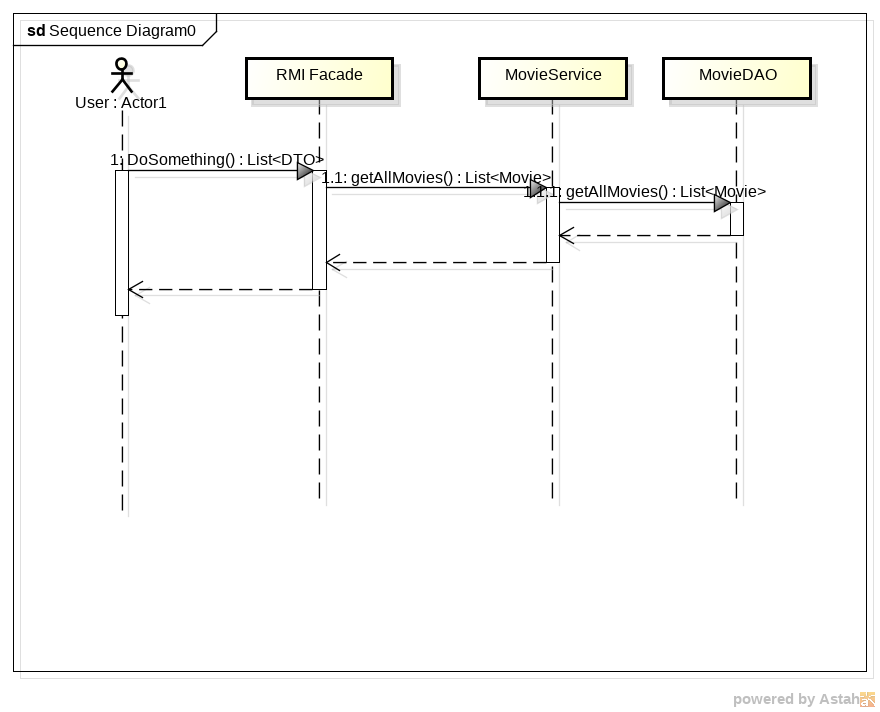
\includegraphics[scale=0.6]{./archan1.png}
 % archan1.png: 880x712 pixel, 96dpi, 23.28x18.84 cm, bb=0 0 660 534
\end{figure}
\pagebreak
\section*{Aufgabe 2}
Für die Integration der RIA Applikation auf der Serverseite müssen zusätzliche Komponenten
implementiert werden. Zeichnen sie in einem Diagramm kann die gesamte Serverapplikation mit den
unterschiedlichen Schichten/Layer und den verschiedenen Client-Applikationen:
\begin{figure}[h]
 \centering
 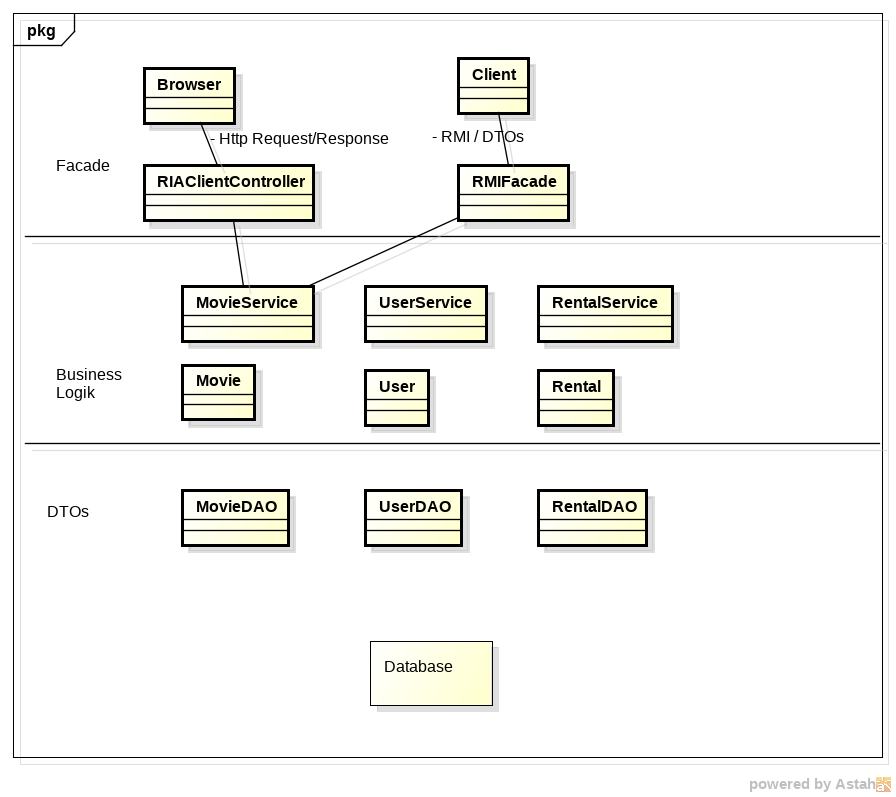
\includegraphics[scale=0.6]{./archan2.png}
 % archan1.png: 880x712 pixel, 96dpi, 23.28x18.84 cm, bb=0 0 660 534
\end{figure}
\section*{Aufgabe 3}
\begin{lstlisting}
	@Controller #1
	public class RIAClientController {
		@ResponseBody #2
		@RequestMapping(value="/movies", method = RequestMethod.GET,
		produces = "application/json")#3
		public List<MovieDTO> getMovies() {#4
			...
		}
	}
\end{lstlisting}
\begin{enumerate}
 \item Der RiaClientController wird über diese Annotation als SpringBean im Speziellen als PageController während das 
ComponentScan beim Bootstrap erkannt.
\item Mut dieser Annotation wird die Response der Methode beschreiben.
\item Mit dem Requestmappng wird die methode an den Http Request webapp/movies gemappt falls der Http Request eine Get 
Methode ist. Die Methode selber wird JSON als Response erzeugen
\item Normale Methode.
\end{enumerate}

\chapter{Extra Code Snippets}
\begin{lstlisting}[caption=JNDI Lookup Helper]
	package com.ibytecode.client;

	import javax.naming.Context;
	import javax.naming.NamingException;

	import com.ibytecode.business.HelloWorld;
	import com.ibytecode.businesslogic.HelloWorldBean;
	import com.ibytecode.clientutility.ClientUtility;

	public class EJBApplicationClient {

		public static void main(String[] args) {
			HelloWorld bean = doLookup();
			System.out.println(bean.sayHello()); // 4. Call business logic
		}

		private static HelloWorld doLookup() {
			Context context = null;
			HelloWorld bean = null;
			try {
				// 1. Obtaining Context
				context = ClientUtility.getInitialContext();
				// 2. Generate JNDI Lookup name
				String lookupName = getLookupName();
				// 3. Lookup and cast
				bean = (HelloWorld) context.lookup(lookupName);

			} catch (NamingException e) {
				e.printStackTrace();
			}
			return bean;
		}

		private static String getLookupName() {
			/*
			The app name is the EAR name of the deployed EJB without .ear suffix.
			Since we haven't deployed the application as a .ear,
			the app name for us will be an empty string
			*/
			String appName = "";

			/* The module name is the JAR name of the deployed EJB
			without the .jar suffix.
			*/
			String moduleName = "HelloWorldSessionBean";

			/*AS7 allows each deployment to have an (optional) distinct name.
			This can be an empty string if distinct name is not specified.
			*/
			String distinctName = "";

			// The EJB bean implementation class name
			String beanName = HelloWorldBean.class.getSimpleName();

			// Fully qualified remote interface name
			final String interfaceName = HelloWorld.class.getName();

			// Create a look up string name
			String name = "ejb:" + appName + "/" + moduleName + "/" +
			distinctName    + "/" + beanName + "!" + interfaceName;

			return name;
		}
	}
\end{lstlisting}
\begin{lstlisting}[caption=Stateful Bean]
 package ch.fhnw.eaf.cart.bean;

import javax.ejb.Remote;

@Remote
public interface Cart {
   public void   initialize(String owner);

   public void   add   (double amount);
   public void   remove(double amount);
   public double getTotal();
   public void   addTax();

   public void   close();
}

package ch.fhnw.eaf.cart.bean;

import javax.annotation.PostConstruct;
import javax.annotation.PreDestroy;
import javax.ejb.PostActivate;
import javax.ejb.PrePassivate;
import javax.ejb.Remove;
import javax.ejb.Stateful;
import javax.inject.Inject;

import org.jboss.ejb3.annotation.Cache;

import ch.fhnw.eaf.calculator.bean.Calculator;


@Stateful
//@Interceptors(ch.fhnw.eaf.tools.LogInterceptor.class)
@Cache("small") // JBoss specific
//@StatefulTimeout(value=5, unit=TimeUnit.SECONDS)
public class CartBean implements Cart {
	
	@Inject
	private Calculator calc;
	
	private String owner;
	public void initialize(String owner){log("initialize");
		if(owner == null) throw new IllegalArgumentException();
		this.owner = owner;
	}

	private double total;
	private boolean taxAdded = false;
	
	public void add(double amount){log("add");
		if(owner == null || taxAdded ) throw new IllegalStateException();
		total += amount;
	}
	public void remove(double amount){log("remove");
		if(owner == null || taxAdded ) throw new IllegalStateException();
		total -= amount;
	}
	public double getTotal(){log("getTotal");
		if(owner == null ) throw new IllegalStateException();
		return total;
	}
	public void addTax(){log("addTax");
		if(owner == null || taxAdded ) throw new IllegalStateException();
		total = calc.sum(total, calc.product(total, calc.quotient(8.0, 100)));
		taxAdded = true;
	}

	@Remove
	public void close() { log("close called"); }

	@PreDestroy
	private void preDestroy(){log("preDestroy called");	}

	@PrePassivate
	private void prePassivate(){log("prePassivate called"); }

	@PostActivate
	private void postActivate(){log("postActivate called");	}
	
	@Override
	public void finalize(){log("finalize called");}

	public CartBean(){log("constructor called"); }

	@PostConstruct
	private void init(){log("postConstruct called");
		System.out.println(calc);
		System.out.println(System.identityHashCode(calc));
		System.out.println(calc.getClass().getName());
	}

	private void log(String msg){
		System.out.println(this.getClass().getSimpleName()+"@"
				+System.identityHashCode(this)
				+" "+msg);
	}
	
}
\end{lst}

\begin{lst}[caption=Stateless Bean]
	package ch.fhnw.eaf.calculator.bean;

	import javax.ejb.Local;

	@Local
	public interface Calculator {
		double sum(double x, double y);
		double difference(double x, double y);
		double product(double x, double y);
		double quotient(double x, double y);

		void incrementCounter();
	}
	package ch.fhnw.eaf.calculator.bean;

	import javax.annotation.PostConstruct;
	import javax.annotation.PreDestroy;
	import javax.ejb.Stateless;

	@Stateless
	public class CalculatorBean implements Calculator {
		private int counter = 0;

		public void incrementCounter(){
			log("incrementCounter: counter "+ counter++);
		}

		public double sum(double x, double y) {
			log("sum called");
			try { Thread.sleep(5000); }
			catch (Exception e) {}
			return x + y;
		}

		public double difference(double x, double y) { log("difference"); return x - y; }
		public double product(double x, double y) {	log("product"); return x * y;}
		public double quotient(double x, double y) { log("quotient"); return x / y;}


		public CalculatorBean(){log("constructor called");}

		@PostConstruct
		private void init(){log("init called");}

		@PreDestroy
		public void remove(){log("remove called");}

		@Override
		public void finalize(){log("finalize called");}

		private void log(String msg){
			System.out.println(this.getClass().getSimpleName()+"@"
			+System.identityHashCode(this)+" "+msg);
		}
	}
\end{lst}
\begin{lst}[caption=Client]
	public class Client2 {
		public static void main(String[] args) throws Exception {
			InitialContext ctx = new InitialContext();
			final String JNDI_NAME = "cart/CartBean!ch.fhnw.eaf.cart.bean.Cart";

			Cart cart = (Cart) ctx.lookup(JNDI_NAME);

			cart.initialize("User1");

			cart.add(44);
			cart.add(112);

			Thread.sleep(20 * 1000);

			cart.addTax();
			System.out.println("total = " + cart.getTotal());

			cart.close();
		}
	}
\end{lstlisting}

\end{document}
